\documentclass{beamer}
\usepackage[utf8]{inputenc}
\usepackage{graphicx} % picturing
\usepackage{cite}
\usepackage{caption}
\usepackage{fancybox}
\usepackage{natbib}
\usepackage{cite}
\usepackage{animate}
\usepackage[utf8]{inputenc}
\usepackage[ngerman]{babel}
\usepackage{graphicx}
\usepackage{color}
\usepackage{float}

\usepackage[ruled,noline]{algorithm2e}
\providecommand{\SetAlgoLined}{\SetLine}
\providecommand{\DontPrintSemicolon}{\dontprintsemicolon}

%quotatation with source
\def\signed #1{{\leavevmode\unskip\nobreak\hfil\penalty50\hskip2em
  \hbox{}\nobreak\hfil(#1)%
  \parfillskip=0pt \finalhyphendemerits=0 \endgraf}}
\newsavebox\mybox
\newenvironment{aquote}[1]
  {\savebox\mybox{#1}\begin{quote}}
  {\signed{\usebox\mybox}\end{quote}}

\setbeamercovered{transparent}

%\usetheme{Pittsburgh}
\usetheme{AnnArbor}
%\usecolortheme{crane}
\usecolortheme{beaver}
\beamertemplatenavigationsymbolsempty
\setbeamertemplate{itemize items}[default]
\setbeamertemplate{enumerate items}[default]
\setbeamertemplate{sections/subsections in toc}[circle]
\setbeamercolor{section number projected}{bg=darkgray,fg=white}
\setbeamercolor{enumerate item}{fg=darkgray}
\setbeamercolor{enumerate subitem}{fg=darkgray}
\setbeamercolor{enumerate subsubitem}{fg=darkgray}
\setbeamercolor{itemize item}{fg=darkgray}
\setbeamercolor{itemize subitem}{fg=darkgray}
\setbeamercolor{itemize subsubitem}{fg=darkgray}
\setbeamercolor{caption name}{fg=darkgray}


\captionsetup[figure]{font=scriptsize}

\setbeamertemplate{footline}
  {%
    \begin{beamercolorbox}[ht=2.5ex,dp=1.125ex,%
      leftskip=.3cm,rightskip=.3cm plus1fil]{author in head/foot}%
      \leavevmode{\usebeamerfont{author in head/foot}\insertshortauthor}%
      \hfill%
      {\usebeamerfont{institute in head/foot}\usebeamercolor[fg]{institute in head/foot}\insertshortinstitute}%
    \end{beamercolorbox}%
    \begin{beamercolorbox}[ht=2.5ex,dp=1.125ex,%
      leftskip=.3cm,rightskip=.3cm plus1fil]{title in head/foot}%
      \leavevmode{\usebeamerfont{title in head/foot}\insertshorttitle}%
      \hfill%
      %{\usebeamerfont{pagecounter in head/foot}\usebeamercolor[fg]{pagecounter in head/foot}\[~\thepage\]}%
      {\usebeamerfont{pagecounter in head/foot}\usebeamercolor[fg]{pagecounter in head/foot}\lbrack~\insertframenumber~\rbrack}%
    \end{beamercolorbox}%
    \begin{beamercolorbox}[colsep=1.5pt]{lower separation line foot}	
    \end{beamercolorbox}
  }


\title[BacArena]{\texttt{BacArena}: Simulation of Interactions in Microbial Communities using Genome-wide Metabolic Reconstructions}
  \author[Eugen Bauer, Johannes Zimmermann]{Eugen Bauer, Johannes Zimmermann\\ \small{\{eugen.bauer, zimmermann.johannes\}@uni-jena.de}}
\institute{Universit\"at Jena}
\date{23.10.2013}
\begin{document}


\frame{
\titlepage
}

\frame{
  \frametitle{Agent based modeling}
  \begin{itemize}
  \setlength{\itemsep}{20pt}
    \item Grid
    \item Substrate
    \item Movement
    \item Diffusion
  \end{itemize}
}

\frame{
  \frametitle{Algorithmic overview}
\begin{algorithm}[H]
  \caption{Main model iterations called by \texttt{diffbac.R} with different functions applied to bacterial agents and metabolite.}
  \SetAlgoLined
  \For{number of iterations}{
    \emph{diffusion}()\;
    \For{number of bacteria}{
      \emph{fba}()\;
      \emph{movement}()\;
      \emph{growth}()\;
    }
  }
  \label{alg:mainloop}
  \end{algorithm}
}

\frame{
  \frametitle{Rules applied to each agent}
  \begin{itemize}
  \setlength{\itemsep}{20pt}
    \item species specific fba calculations with substrate concentrations as contraints
    \item diffusion of substrates to neighbours with lower concentrations
    \item random movement on the grid environment
    \item growth according to accumulated biomass
  \end{itemize}
}

\frame{
  \frametitle{Some Feature}
  \begin{itemize}
  \setlength{\itemsep}{20pt}
    \item Reproducible Simulations
    \begin{itemize}
    		\item setting seed for random number generation
    \end{itemize}
    \item Modularity ($\rightarrow$ easily extendable)
    \begin{itemize}
    		\item division of different functions
    		\item additional SBML models
    \end{itemize}
  \end{itemize}

}

\frame{
  \frametitle{Growth of \textit{Escherichia coli}}
  \begin{columns}
  \centering
  \begin{column}{.48\textwidth}

    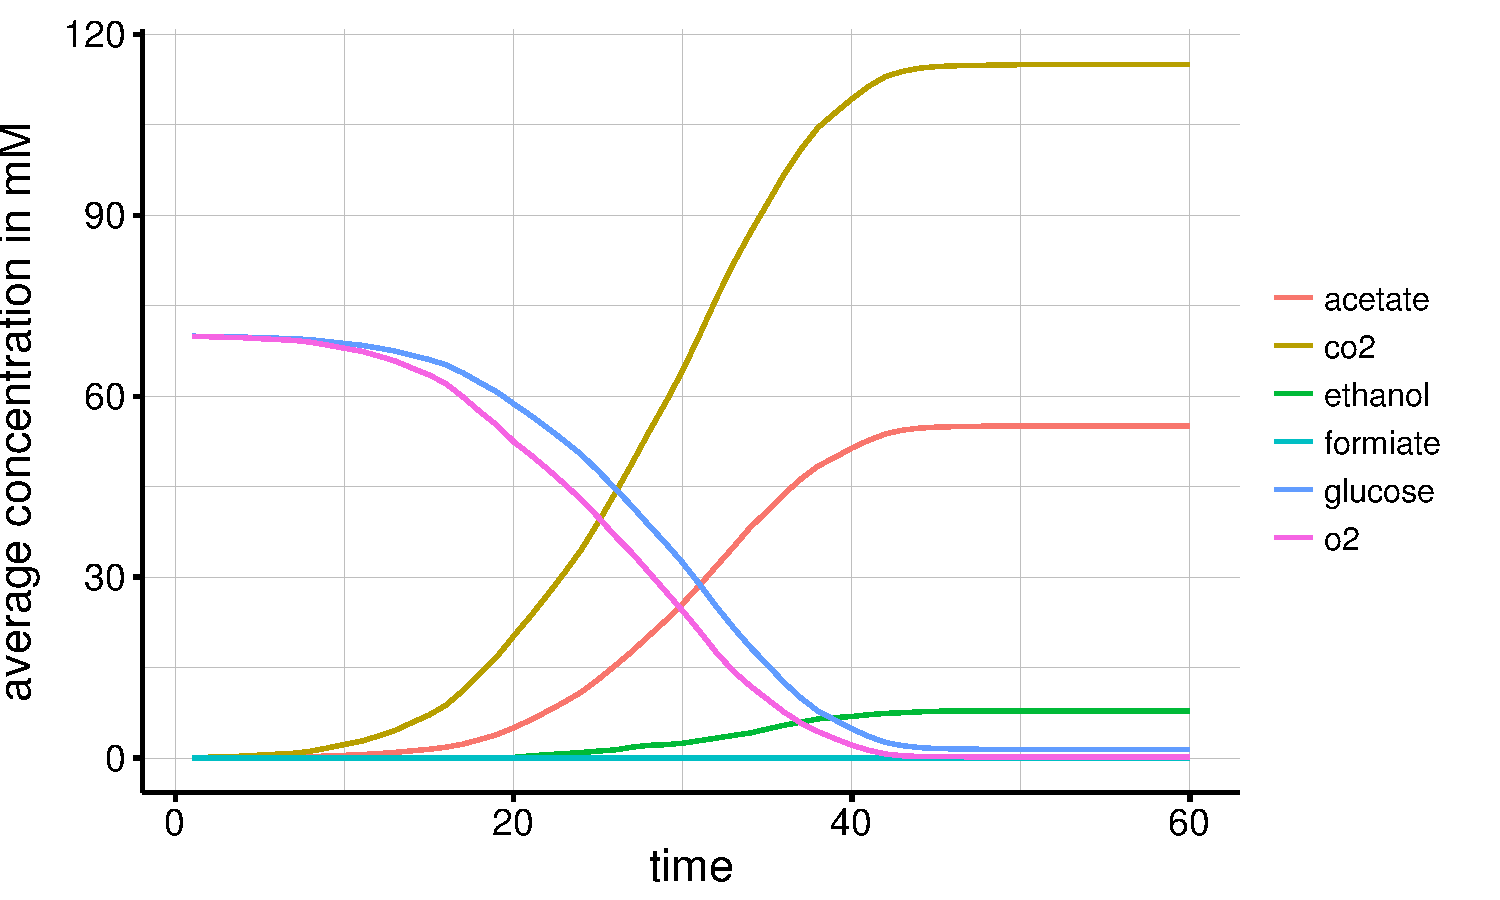
\includegraphics[width=\textwidth]{../results/img/Bcoli_20x20_seed911_subs.pdf}
  \end{column}
  \hfill
  \begin{column}{.48\textwidth}

    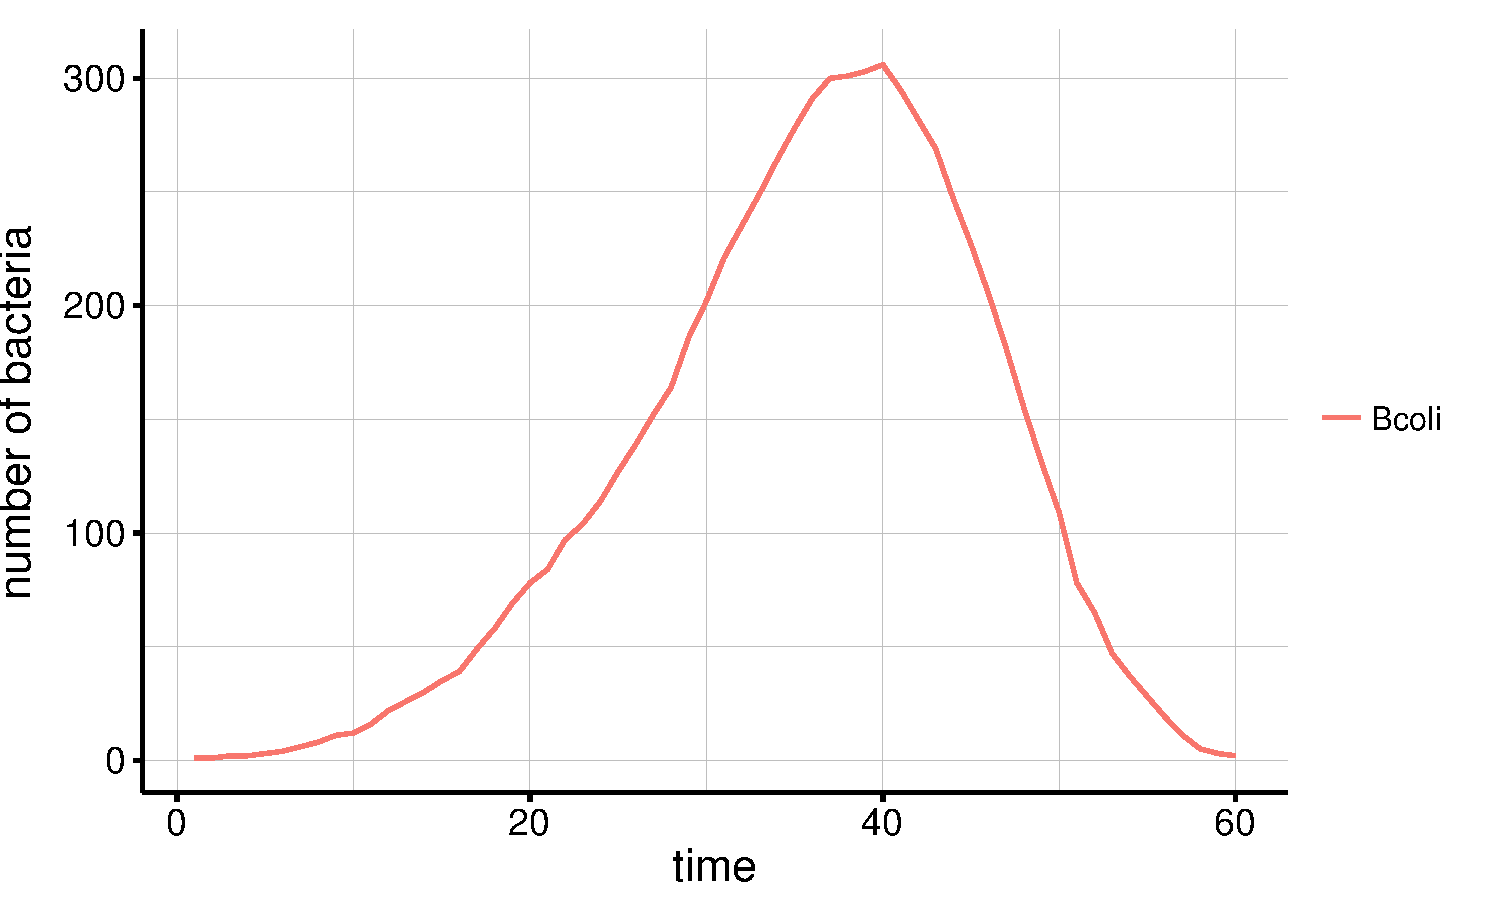
\includegraphics[width=\textwidth]{../results/img/Bcoli_20x20_seed911_growth.pdf}
  \end{column}
  \end{columns}
}


\frame{
  \frametitle{Growth of \textit{Methanosarcina barkeri}}
  \begin{columns}
  \centering
  \begin{column}{.48\textwidth}

    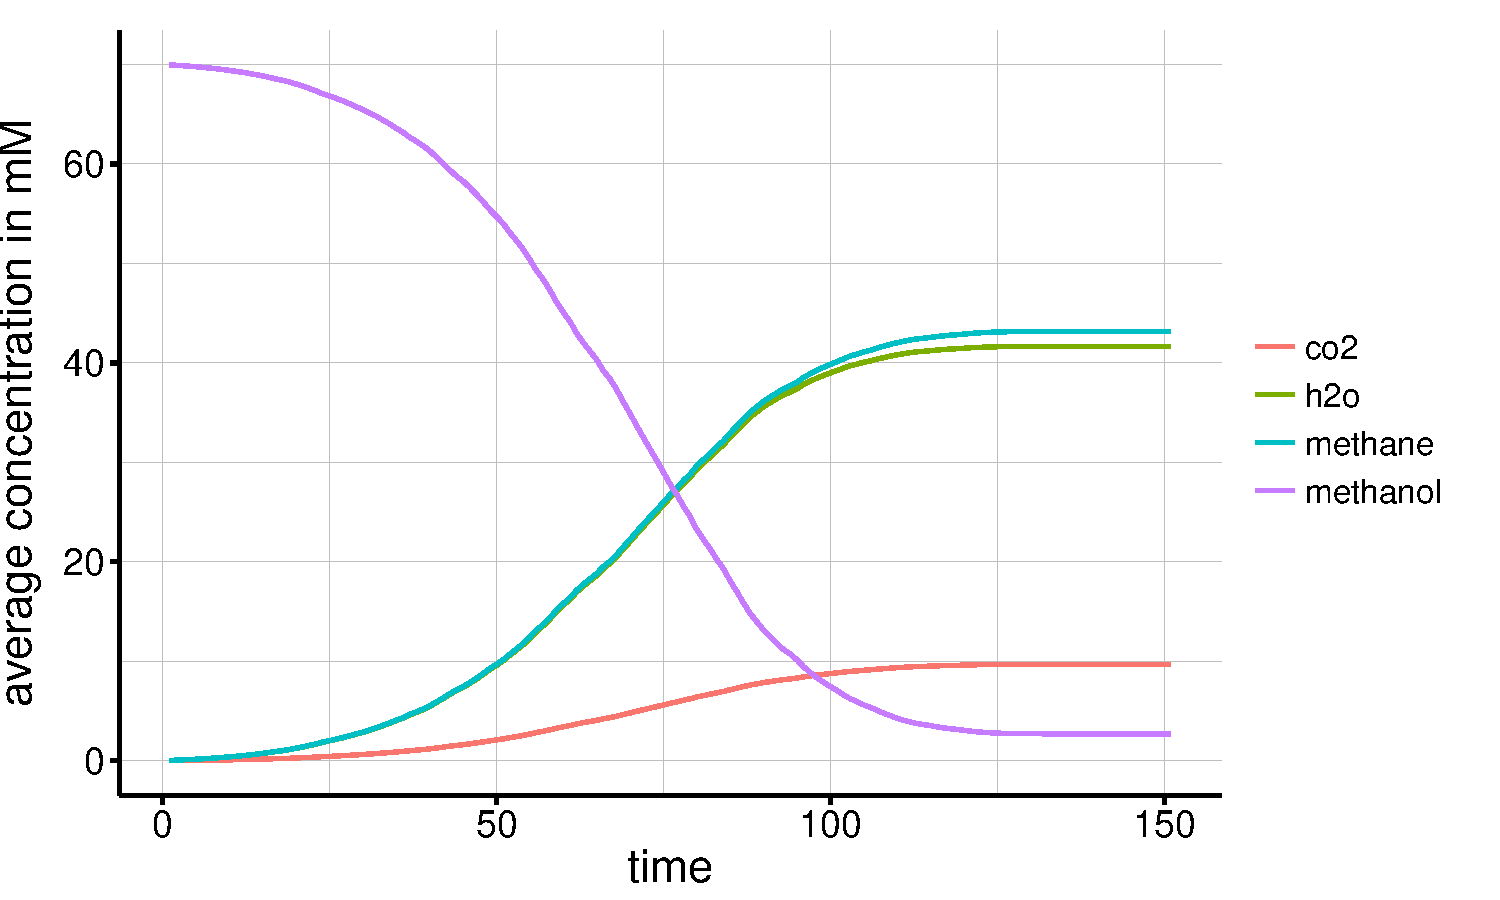
\includegraphics[width=\textwidth]{../results/img/barkeri_20x20_seed9659_subs.pdf}
  \end{column}
  \hfill
  \begin{column}{.48\textwidth}

    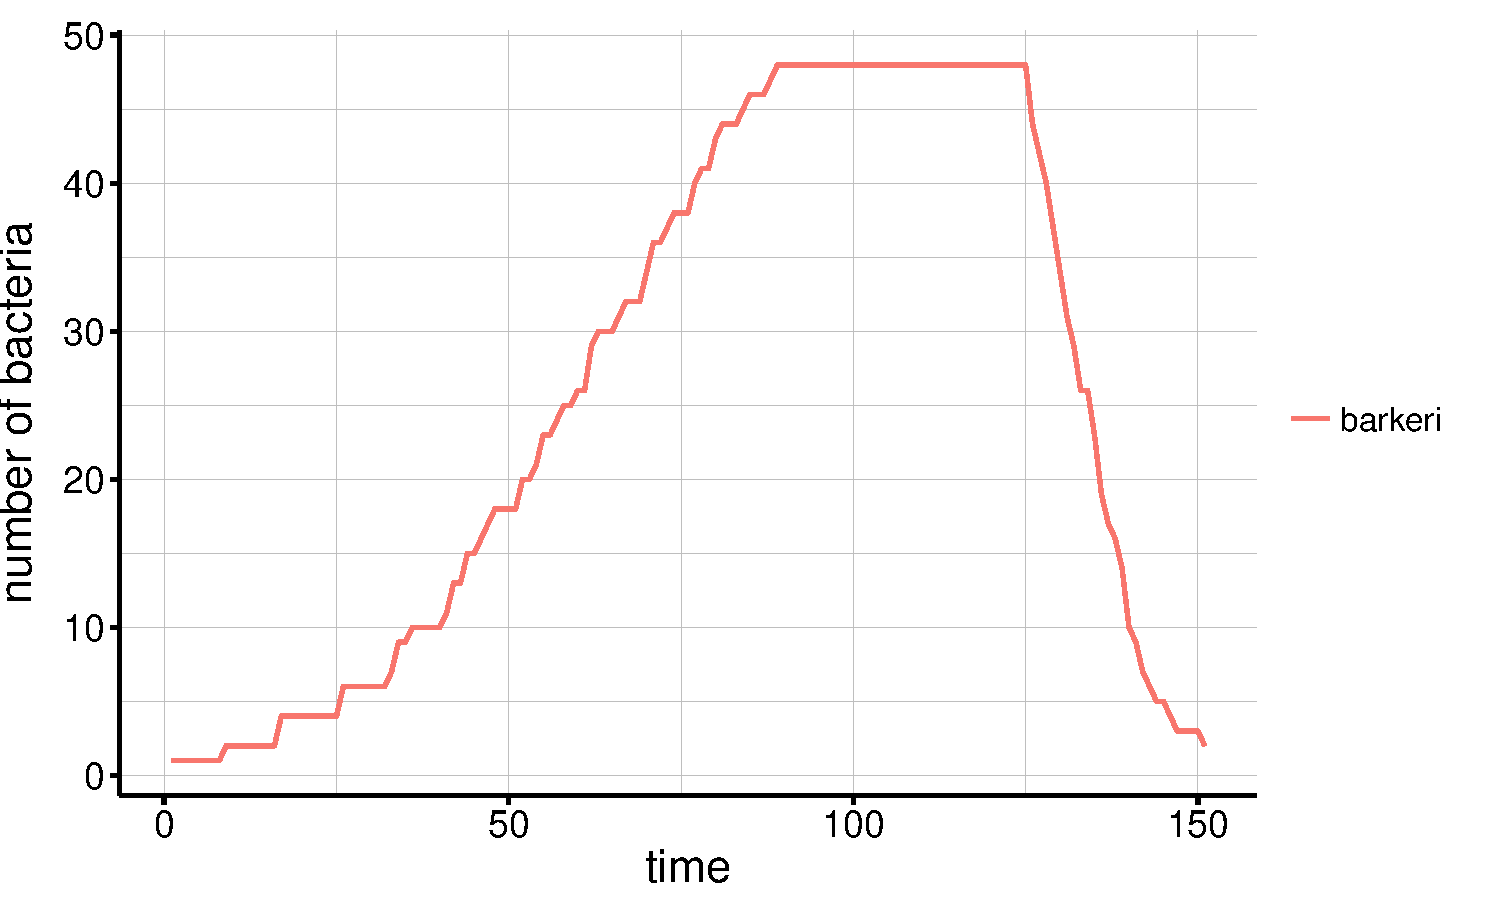
\includegraphics[width=\textwidth]{../results/img/barkeri_20x20_seed9659_growth.pdf}
  \end{column}
  \end{columns}
}

\frame{
  \frametitle{Growth of \textit{Clostridium beijerinckii}}
  \begin{columns}
  \centering
  \begin{column}{.48\textwidth}

    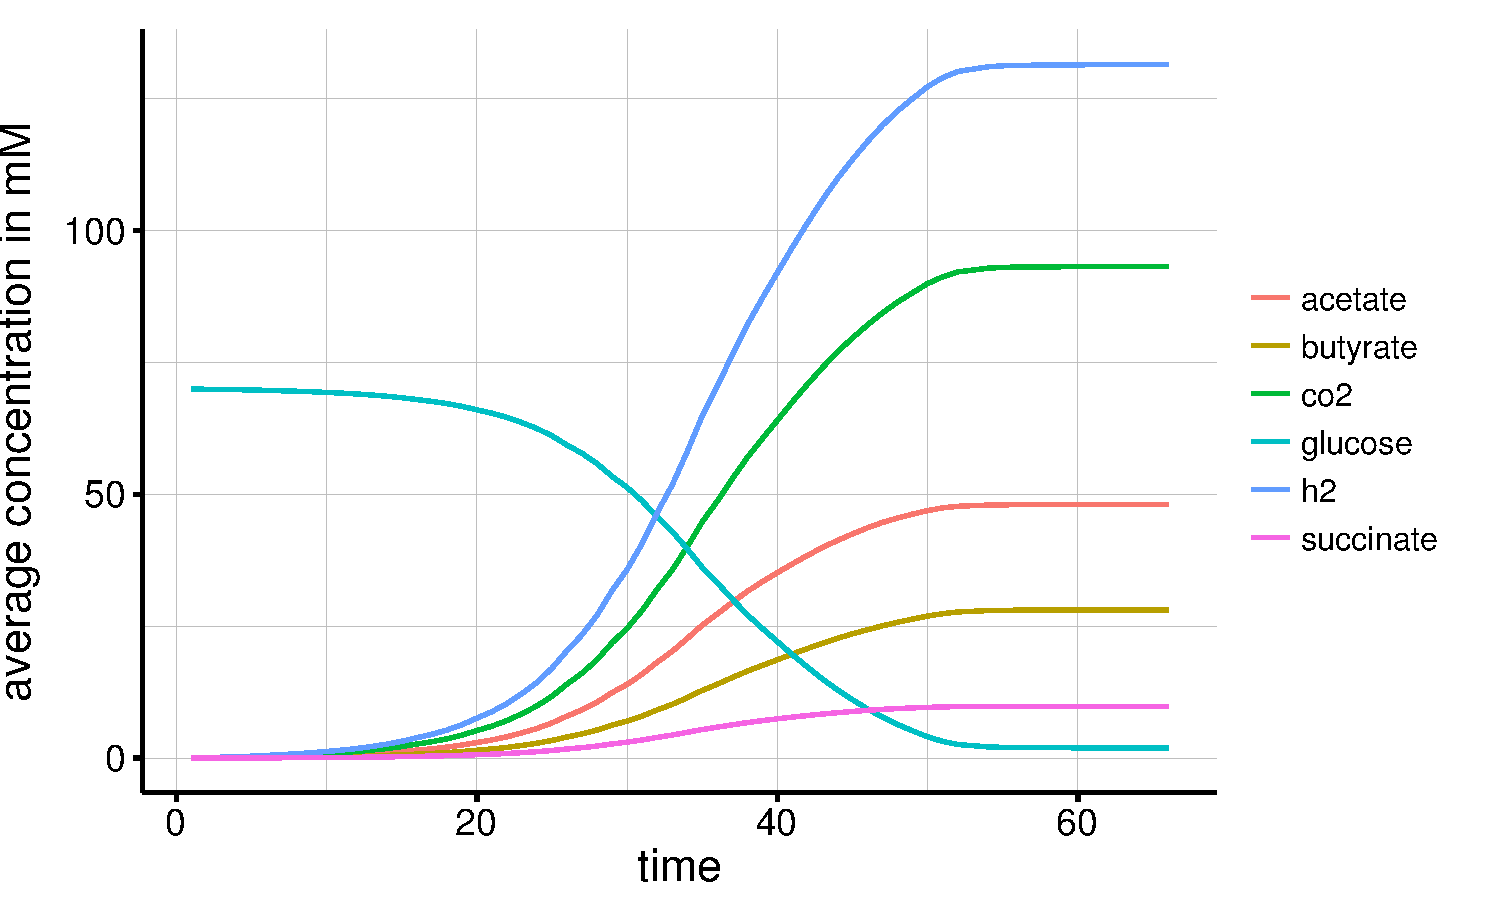
\includegraphics[width=\textwidth]{../results/img/beijerinckii_20x20_seed943_subs.pdf}
  \end{column}
  \hfill
  \begin{column}{.48\textwidth}

    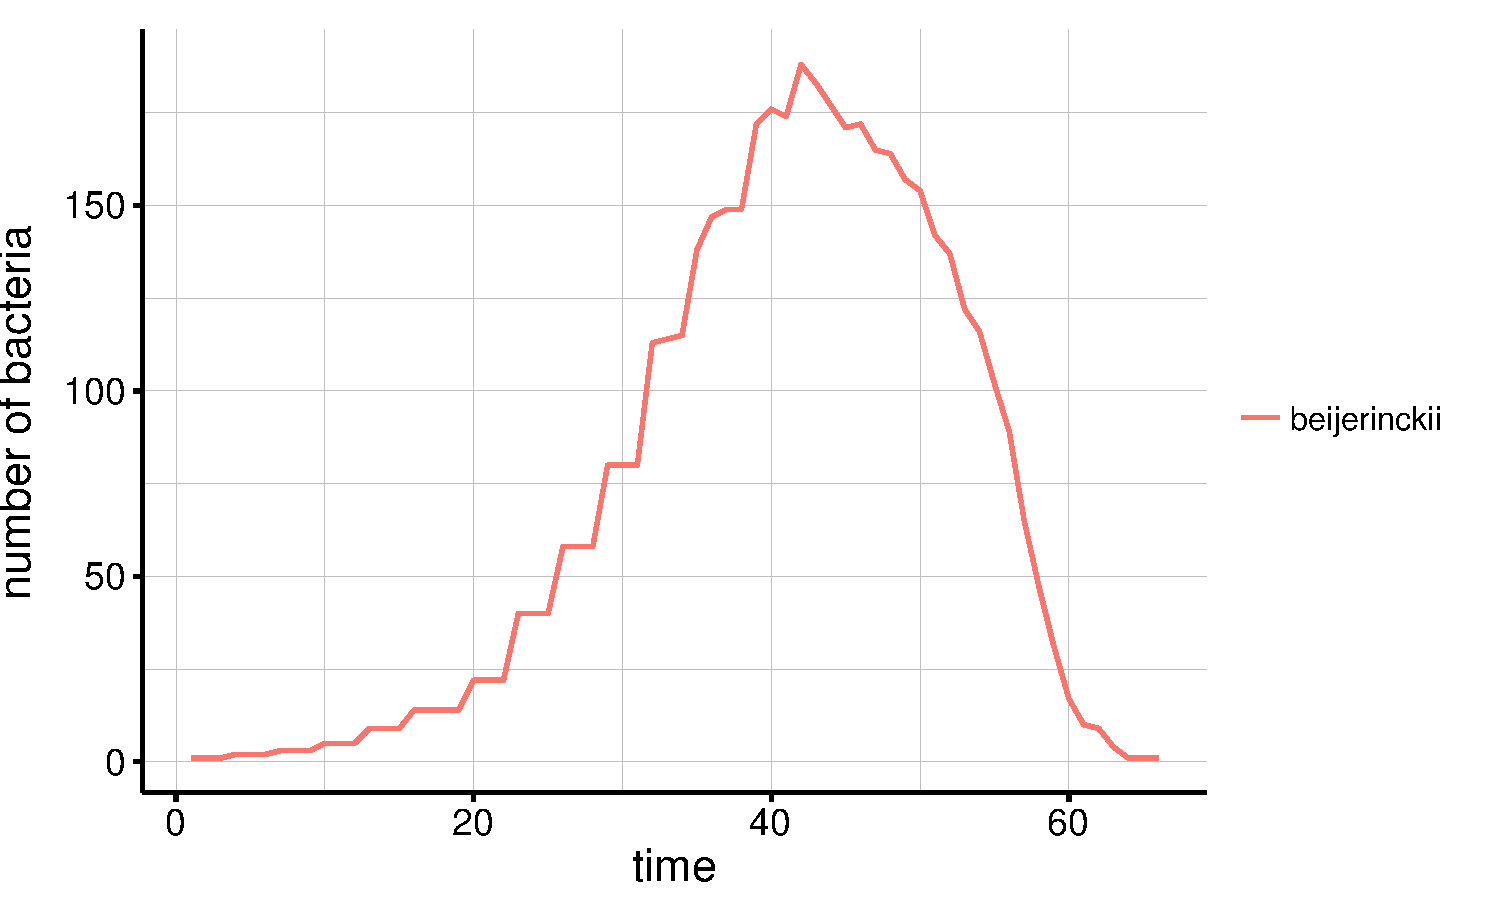
\includegraphics[width=\textwidth]{../results/img/beijerinckii_20x20_seed943_growth.pdf}
  \end{column}
  \end{columns}
}

\frame{
  \frametitle{Growth of \textit{Escherichia coli}}
  \begin{columns}
  \centering
  \begin{column}{.48\textwidth}

    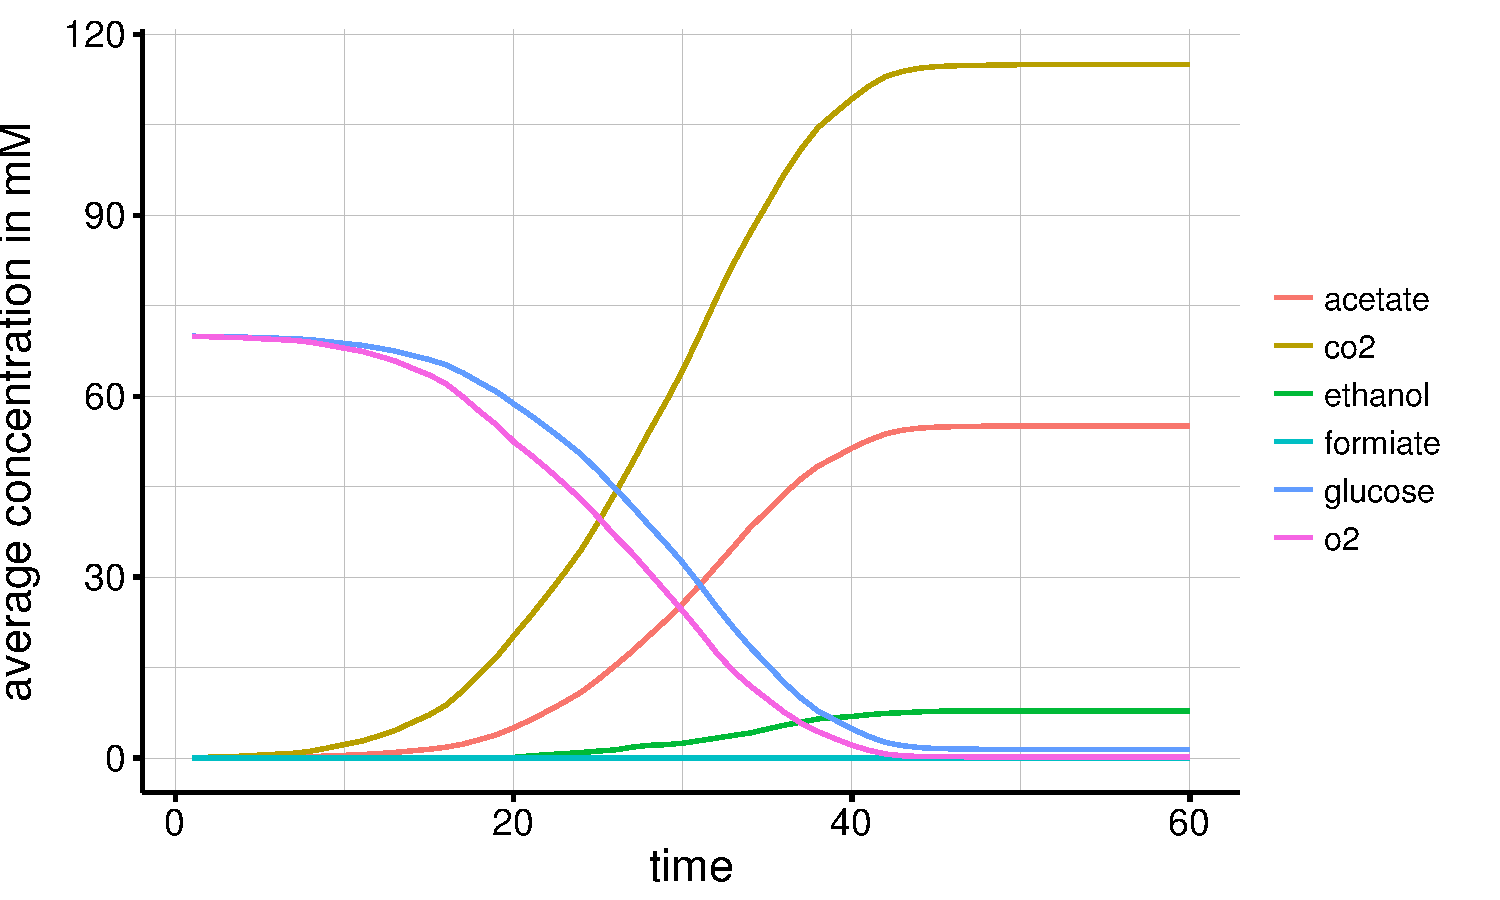
\includegraphics[width=\textwidth]{../results/img/Bcoli_20x20_seed911_subs.pdf}
  \end{column}
  \hfill
  \begin{column}{.48\textwidth}

    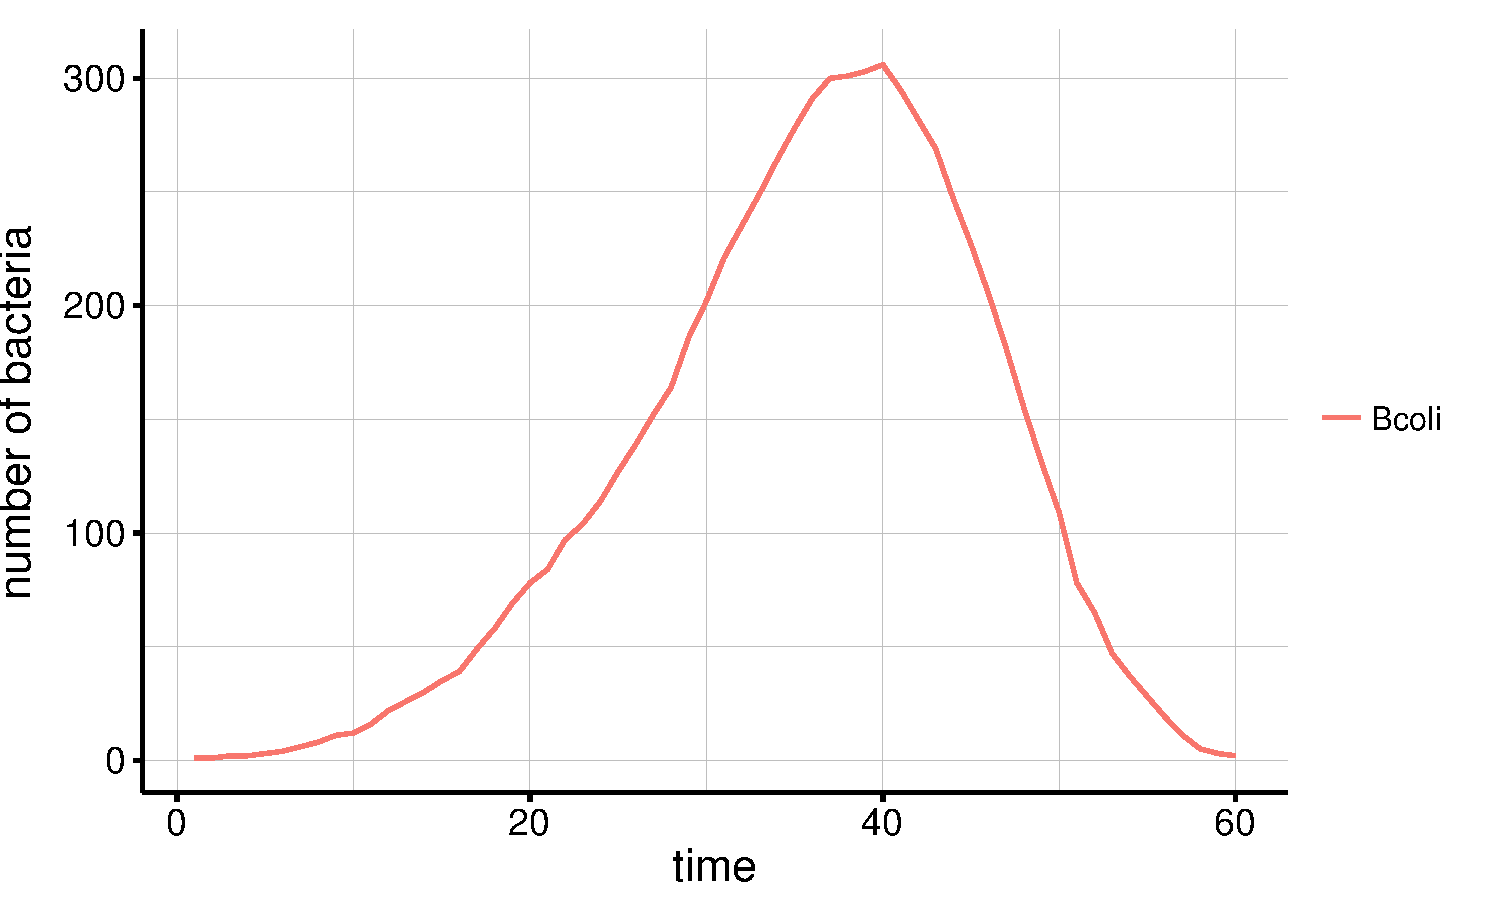
\includegraphics[width=\textwidth]{../results/img/Bcoli_20x20_seed911_growth.pdf}
  \end{column}
  \end{columns}
}


\end{document}


\frame{
  \frametitle{}
}
  \begin{figure}
    \centering
    \includegraphics[height=0.85\textheight]{./bacarena1.pdf}
  \end{figure}
}
\frame{
  \frametitle{BacArena: Methanosarcina barkeri}
  \begin{figure}
    \centering
    \includegraphics[height=0.85\textheight]{./bacarena2.pdf}
  \end{figure}
